

\documentclass{beamer}
\setbeamertemplate{caption}{\raggedright\insertcaption\par}
 
\usepackage[utf8]{inputenc}

\usetheme{Boadilla}
\usecolortheme{default}
\usepackage{dsfont}
\usepackage{multirow}
\usepackage{tikz}
\usetikzlibrary{bayesnet}
\usepackage{amsmath}
\usepackage{graphicx}
\usepackage{subcaption}

\newcommand{\ci}{\mathrel{\text{\scalebox{1.07}{$\perp\mkern-10mu\perp$}}}}



 
%Information to be included in the title page:
\title[] %optional
{Robustness against Distribution Shift using Causal Models}
 
%\subtitle{A short story }
 
%\author[Wang, Webb, Rainforth] % (optional, for multiple authors)
%{Benjie Wang, Stefan Webb, Tom Rainforth}

 
 
\date[03/03/2020] % (optional)
{}
 


\AtBeginSection[]
{
  \begin{frame}
    \frametitle{Table of Contents}
    \tableofcontents[ 
currentsection,
currentsubsection
] 
  \end{frame}
}

\AtBeginSubsection[]
{
    \begin{frame}
        \frametitle{Table of Contents}
        \tableofcontents[currentsection,currentsubsection]
    \end{frame}
}

 
\begin{document}
 
\frame{\titlepage}

 

 
\section{Recap}

\begin{frame}
\frametitle{Causality}
\begin{itemize}
	\item Causality is the study of the underlying structure of a system;
	\bigskip
	
	\item Through studying causality and causal models, we can:
	\begin{itemize}
		\item Answer questions about how a system responds to \textbf{changes} in its mechanisms;
		\item Specify causal relationships that are more \textbf{stable} and more fundamental than generic statistical relationships.
	\end{itemize}
	
	\bigskip
	\item A model assigns truth values to statements about the system; a causal model assigns truth values to causal statements/queries
\end{itemize}
\note[]{
Study of the generative process. Not just the distribution over observed variables.

If a small part of the system changed, our statistical/ML models would be useless and we'll have to gather loads of data in the new environment and learn it all again.

Causal relationships are how humans think - and for good reason, it's a compact and STABLE representation. If we change one part, the others shouldn't change. "disentangled" the system.

From the perspective of AI, we can use statistical models, i.e. probability distributions, make predictions about the world (ML, e.g. BNNs) p(y|x), model-based RL p(s'|s, a), learn state-action value functions in RL (in distributional RL, p(v|s, a). (both useful for autonomous agents and for general data science). Imagine what we could do if in addition we knew about:
- ML: what would have happened in the population had these people stopped smoking?
- RL/agents: what would have happened the car had slowed down, given what we know about what actually happened? or alternatively, what would happen if instead of following our policy, we chose an alternative action (off-policy)?
}
\end{frame}

\begin{frame}
\frametitle{Causal Bayesian Networks}
\textbf{Causal Bayesian Networks} are a means for representing a set of interventional distributions, consisting of:
\pause
\begin{itemize}
	\item A directed acyclic graph (DAG) G:
\end{itemize}
	\begin{center}
	\tikz{ %
        \node[latent] (x_5) {$x_5$} ; %
        \node[latent, left=of x_5, yshift=0.8cm] (x_3) {$x_3$} ; %
        \node[latent, left=of x_5, yshift=-0.8cm] (x_4) {$x_4$} ; %
        \node[latent, left=of x_3, yshift=0cm] (x_2) {$x_2$} ; %
        \node[latent, left=of x_4, yshift=0cm] (x_1) {$x_1$} ; %
        \edge {x_3,x_4} {x_5} ; %
        \edge {x_2} {x_3} ;
        \edge {x_3} {x_4} ;
        \edge {x_1} {x_4} ;
        \edge {x_1} {x_2} ;
      }
     \end{center}
     \pause
\begin{itemize}
	\item A probability distribution $P(x| pa(x))$ for every node $x$ in the DAG
\end{itemize}
\pause

\bigskip
The joint probability distribution is then $P(x_1, ..., x_N) = \prod_{i} P(x_i | pa(x_i))$.

\note[]{
This looks familiar... so how can the same DAG + parent-child probability distributions define a whole set of interventional distributions?
}
\end{frame}

\begin{frame}
\frametitle{Principle of Independent Causal Mechanisms}
The \textbf{ICM principle} states that the individual causal mechanisms of a systems' causal generative process do not:
\begin{itemize}
\pause
	\item \textit{inform} each other
	\item \textit{influence} each other
\end{itemize}

To mimic this in our causal model, we derive interventional distributions by making the necessary intervention and leaving all other mechanisms.

Example: $P_{X_4 = x'} (x_1, ..., x_5)$

\begin{center}
	\tikz{ %
        \node[latent] (x_5) {$x_5$} ; %
        \node[latent, left=of x_5, yshift=0.8cm] (x_3) {$x_3$} ; %
        \node[latent, left=of x_5, yshift=-0.8cm] (x_4) {$x_4$} ; %
        \node[latent, left=of x_3, yshift=0cm] (x_2) {$x_2$} ; %
        \node[latent, left=of x_4, yshift=0cm] (x_1) {$x_1$} ; %
        \edge {x_3,x_4} {x_5} ; %
        \edge {x_2} {x_3} ;
        \edge {x_1} {x_2} ;
      }
\end{center}

$P_{X_4 = x'} (x_1, ..., x_5) = P(x_2|x_1) P(x_3|x_2) \mathds{1}_{x_4 = x'} P(x_5|x_3, x_4)$

\note[] {
Of course, here we are just making this assumption in our model and hoping that it reflects reality. But it is certainly reasonable.

This is why causal relationships are stable. By changing one mechanism in the generative process, we can completely mess up a probability distribution. Meanwhile the actual causal generative process has only changed slightly. We wish to mimic this in our models.

"Disentangled"
}
\end{frame}

\section{Introduction}
\begin{frame}
\frametitle{Problem Setting}
\textbf{Problem}: Machine learning models are not robust to changes in the data generating process (DGP) from train to test time (\textit{distribution shift}).
\bigskip

\begin{itemize}
	\item Deployment of medical treatments in different hospitals;
	\item Autonomous vehicles in harsh weather conditions (snow, rain, etc.);
	\item Variants of environments in RL;
	\item Different dialects in language;
\end{itemize}

\bigskip
How do we define what kinds of changes our machine learning models should be robust to?

\medskip
How do we actually achieve this robustness?

\note[]{
Violates the i.i.d. assumption, which pervades machine learning, e.g. replay in RL.
These are all things which come naturally to humans.

It doesn't make sense to talk about arbitrary changes.
}
\end{frame}

\subsection{Types of distribution shift}
\begin{frame}
\frametitle{What might vary?}

In a typical machine learning problem, we wish to predict a label or target $Y$, given covariates $X$. There are two basic possible causal graphs:



\begin{figure}[ht]
\begin{subfigure}{.4\linewidth}
  \centering
  % include first image
  \tikz{ %
        \node[obs] (Y1) {$Y$} ; %
        \node[obs, left=of Y1, yshift=0cm] (X1) {$X$} ; %
        \node[factor, left=of X1, yshift=0cm] (S1) [label=$S_X$] {};
        \node[factor, yshift=1cm] (S2) [label=$S_Y$] {};
        
        \edge {X1} {Y1} ;
        \edge {S1} {X1} ;
        \edge {S2} {Y1} ;
      }
  \caption{$p_X, p_{Y|X}$}
  \label{fig:sub-first}
\end{subfigure}
\begin{subfigure}{.4\linewidth}
  \centering
  \tikz{ %
        \node[obs] (X2) {$X$} ; %
        \node[obs, left=of X2, yshift=0cm] (Y2) {$Y$} ; %
		\node[factor, left=of Y2, yshift=0cm] (S1) [label=$S_Y$] {};
        \node[factor, yshift=1cm] (S2) [label=$S_X$] {};        
        
        \edge {Y2} {X2} ; %
        \edge {S1} {Y2} ;
        \edge {S2} {X2} ;
      }
  \caption{$p_Y, p_{X|Y}$}
  \label{fig:sub-second}
\end{subfigure}
\label{fig:fig}
\end{figure}

and 4 possible types of distribution shift:

\begin{enumerate}
	\item \textbf{Covariate shift}: $X \to Y$ with $p_X$ changing and $p_{Y|X}$ fixed.
	\item $X \to Y$ with $p_{Y|X}$ changing.
	\item \textbf{Target/label shift}: $Y \to X$ with $p_{Y}$ changing and $p_{X|Y}$ fixed.
	\item $Y \to X$ with $p_{X|Y}$ changing
\end{enumerate}

\note[]{
Examples of b): Clinical diagnosis (disease -> symptoms), Image recognition
Examples of a): 

1) and 3) are sometimes possible without additional assumptions if the dimensionality of $X$ and $Y$ respectively is not too large; in the other 
}
\end{frame}

\begin{frame}
\frametitle{How much does it vary by?}

We need additional assumptions, or restrictions on how much these probability distributions can change.
\bigskip

Approaches to obtaining robust models rely on these assumptions: 
\begin{itemize}
	\item Assume only covariate shift/only label shift occurs
	\item Limit change in $p(Y|X)$ by KL-divergence \cite{Duchi+Namkoong18}
	\item Assume that target environment is "sufficiently" similar to multiple source environments \cite{ZhangEtAl15}
\end{itemize}

\note[]{
DRO
Multi-domain adaption
}
\end{frame}

\begin{frame}
\frametitle{Distribution shift as interventions in DGP}
We reason about changes in the underlying DGP that generates the data.
\begin{center}
\tikz{ %
        \node[obs] (A) {$A$};
        \node[factor, yshift=1.5cm] (S) [label=$S$] {};
        \node[obs, left=of A, yshift=-1.5cm] (C) {$C$};
        \node[latent, left=of A, yshift=1.5cm] (K) {$K$};
        \node[obs, left=of K, yshift=-1.5cm] (T) {$T$};
        
        \edge {S} {A};
        \edge [dashed] {K} {A};
        \edge {A} {C};
        \edge [dashed] {K} {T};
        \edge {T} {C};
      }
\end{center}
Here grey nodes are \textbf{observed}, blank nodes are \textbf{unobserved/latent} and black squares are \textbf{selection variables}. $X = \{A, C\}, Y = \{T\}$.
\medskip

Selection variables represent potential \textit{interventions} on variables which might have their mechanisms changed in the target environment, in this case $p_{A|K}$.
\note[]{
Explain the scenario.

Independence of causal mechanisms

"Unreliable mechanisms"

Why use this framework? 
1) More granular/flexible specification of what might change.  

There is still the question of what sort of interventions to allow. We'll only consider the case where we allow arbitrary interventions, however you can imagine that we could impose further restrictions
}
\end{frame}

\subsection{Defenses}
\begin{frame}
\frametitle{Reactive vs Proactive approaches}
\textbf{Reactive} approaches use some (usually unlabelled) data from the target environment in order to optimize the machine learning model for that domain.

\medskip
\textbf{Proactive} approaches use machine learning models which are agnostic to the specific target environment (within the class of environments satisfying assumptions).

\medskip
We focus on a \textbf{proactive} approach, which has the following advantages:
\begin{itemize}
	\item Do not require any data from the target environment
	\item "One-shot": Achieves performance immediately on first test from target environment
	\item Closer to how humans adapt
\end{itemize}
\end{frame}

\section{Graph Surgery}
\begin{frame}
\frametitle{Motivating example}
\begin{center}
\tikz{ %
        \node[obs] (A) {$A$};
        \node[factor, yshift=1.5cm] (S) [label=$S$] {};
        \node[obs, left=of A, yshift=-1.5cm] (C) {$C$};
        \node[latent, left=of A, yshift=1.5cm] (K) {$K$};
        \node[obs, left=of K, yshift=-1.5cm] (T) {$T$};
        
        \edge {S} {A};
        \edge [dashed] {K} {A};
        \edge {A} {C};
        \edge [dashed] {K} {T};
        \edge {T} {C};
      }
\end{center}

We wish to predict in hospitalized patients whether or not they have \textbf{lung cancer} ($T$), on the basis of \textbf{chest pain symptoms} $C$ and whether or not they take \textbf{aspirin} $A$. 

\smallskip
\textbf{Smoking} $K$ is an \textit{unobserved confounder} which affects the chance of lung cancer and heart disease. Aspirin is taken for the latter.

\smallskip
The policy for prescribing aspirin will differ across hospitals, so we add a selection variable $S$ to represent that this mechanism is \textbf{unreliable}.
\end{frame}

\begin{frame}
\frametitle{Task and Assumptions}
We want an \textbf{estimator} $\hat{P}(T|C, A)$ which performs well under all environments, as specified by the selection variables.

\bigskip
We assume that:
\begin{itemize}
\item The causal graph is known (but not the conditional distributions $p(x|pa(x))$;
\item We know which mechanisms are unreliable;
\end{itemize}

\note[]{
Little informal; we'll discuss formalizing this later
}
\end{frame}

\begin{frame}
\frametitle{Stability}

\textbf{Definition} An estimator $\hat{P}$ is \textit{stable} if it is conditionally independent of all selection variables given its inputs.

\begin{figure}[ht]
\begin{subfigure}{.4\linewidth}
  \centering
  % include first image
\tikz{ %
        \node[obs] (A) {$A$};
        \node[factor, yshift=1.5cm] (S) [label=$S$] {};
        \node[obs, left=of A, yshift=-1.5cm] (C) {$C$};
        \node[latent, left=of A, yshift=1.5cm] (K) {$K$};
        \node[obs, left=of K, yshift=-1.5cm] (T) {$T$};
        
        \edge {S} {A};
        \edge [dashed] {K} {A};
        \edge {A} {C};
        \edge [dashed] {K} {T};
        \edge {T} {C};
      }
  \label{fig:tt}
\end{subfigure}
\begin{subfigure}{.4\linewidth}
  \centering
  \tikz{ %
        \node[obs] (Z) {$Z$} ; %
        \node[obs, left=of Z, yshift=-2cm] (X) {$X$} ; %
		\node[obs, left=of X, yshift=2cm] (Y) {$Y$};
		\node[factor, yshift=1cm] (S) [label=$S$] {};  
        
        \edge {S} {Z} ; %
        \edge {Y} {Z} ;
        \edge {Y} {X} ;
        \edge {Z} {X} ;
      }
  \label{fig:d}
\end{subfigure}
\label{fig:ef}
\end{figure}

Intuitively, this means given the same input, the predictions $\hat{P}$ are independent of which environment we are in.

\note[]{
Go through the 2 examples where the discriminative classifier isn't stable

Of course we don't just want any stable estimator (a random guesser is stable), but the best stable estimator
}
\end{frame}

\begin{frame}
\frametitle{Graph Surgery}
Idea: Remove dependence on environment-varying mechanisms by performing graph surgery.
\pause

\only<1-2>{
\begin{center}
\tikz{ %
        \node[obs] (A) {$A$};
        \node[factor, yshift=1.5cm] (S) [label=$S$] {};
        \node[obs, left=of A, yshift=-1.5cm] (C) {$C$};
        \node[latent, left=of A, yshift=1.5cm] (K) {$K$};
        \node[obs, left=of K, yshift=-1.5cm] (T) {$T$};
        
        \edge {S} {A};
        \edge [dashed] {K} {A};
        \edge {A} {C};
        \edge [dashed] {K} {T};
        \edge {T} {C};
      }
\end{center}
}
\pause

\only<3->{

\begin{center}
\tikz{ %
        \node[obs] (A) {$A$};
        \node[factor, yshift=1.5cm] (S) [label=$S$] {};
        \node[obs, left=of A, yshift=-1.5cm] (C) {$C$};
        \node[latent, left=of A, yshift=1.5cm] (K) {$K$};
        \node[obs, left=of K, yshift=-1.5cm] (T) {$T$};
        
        \edge {A} {C};
        \edge [dashed] {K} {T};
        \edge {T} {C};
      }
\end{center}
}
\pause
$$p(T|C, do(A)) \propto p(T, C|do(A)) \propto p(T) p(C|T, A) $$

\pause
\textbf{Theorem}: Any estimator of the form $P(T|Z, do(X))$ where $X \supseteq M$ is stable.
\note[]{
Note this estimator is now stable, while we have made "the minimal possible change" to the formula so it is still predictive.

$p_{G_{\bar{A}}}(T|C, A)$
Comment on being careful: we are not interested in counterfactual notion here.
}
\end{frame}

\section{Graph Surgery in Semi-Markovian Models}
\begin{frame}
\frametitle{Semi-Markovian Models}

In general, we are concerned with \textbf{Semi-Markovian models}, that is, models where there are unobserved/latent nodes which cause confounding.
\bigskip

The previous example suggested that we should use the interventional distribution:

$$p(T|do(M), O\setminus(M \cup T))$$

\medskip
where $T$ are the target variable(s), $M$ are the mutable variables, and $O$ are the observable variables.

\medskip
However, this runs into two issues:
\end{frame}

\begin{frame}
\frametitle{Semi-Markovian Models}
\framesubtitle{1. Mutable Target}

In some cases, the target itself is mutable:
\only<1>{
\begin{center}
\tikz{ %
        \node[obs] (Z) {$Z$} ; %
        \node[obs, left=of Z, yshift=-2cm] (X) {$X$} ; %
		\node[obs, left=of X, yshift=2cm] (Y) {$Y$};
		\node[factor, yshift=1cm] (SZ) [label=$S_Z$] {};
		\node[factor, left=of X, yshift=3cm] (SY) [label=$S_Y$] {};
		  
        
        \edge {SZ} {Z} ; %
        \edge {SY} {Y} ;
        \edge {Z} {Y} ;
        \edge {Y} {X} ;
        \edge {Z} {X} ;
      }
\end{center}
}
\only<2->{
\begin{center}
\tikz{ %
        \node[obs] (Z) {$Z$} ; %
        \node[obs, left=of Z, yshift=-2cm] (X) {$X$} ; %
		\node[obs, left=of X, yshift=2cm] (Y) {$Y$};
		\node[factor, yshift=1cm] (SZ) [label=$S_Z$] {};
		\node[factor, left=of X, yshift=3cm] (SY) [label=$S_Y$] {};
		  
        \edge {Y} {X} ;
        \edge {Z} {X} ;
      }
\end{center}
}

Here $T = \{Y\}$ and $M = \{Y, Z\}$ are not disjoint.
\medskip

\pause
We use $p_{G_{\bar{T}}}(T|do(M\setminus T), O\setminus M) = p_{G_{\bar{Y}}}(Y|do(Z), X)$ = $p(X|Y, Z)$.
\note[]{
Use scene/animal example

Idea is even though target is mutable, we can still learn about it through its children.
}
\end{frame}


\begin{frame}
\frametitle{Semi-Markovian Models}
\framesubtitle{2. Non-identifiability}
Sometimes it's not possible to evaluate an interventional quantity from observational data.

\begin{center}
\tikz{ %
        \node[obs] (Y) {Y};
        \node[latent, left=of Y, yshift=1.5cm] (Z) {Z};
        \node[obs, left=of Z, yshift=-1.5cm] (X) {X};
        
        \edge {X} {Y};
        \edge [dashed] {Z} {X};
        \edge [dashed] {Z} {Y};
      }
\end{center}

$p(Y|do(X))$ is non-identifiable as we don't know how much of the correlation in $p(Y|X)$ is due to the unobserved confounder.

\medskip
For more complex DAGs we can test for identifiability using the ID algorithm. The idea is that if $p(T|do(M), O\setminus(M \cup T))$ is not identifiable, we try conditioning on a smaller set, i.e. $p(T|do(M), W)$.
\note[]{
ADMG on board
}
\end{frame}

\begin{frame}
\frametitle{Overall Algorithm}
\centering
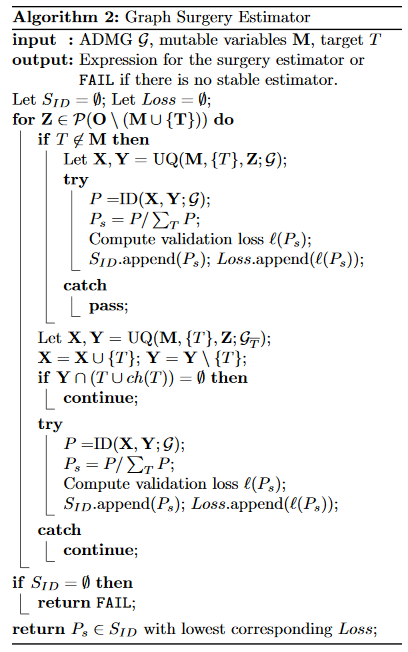
\includegraphics[scale=0.45]{figures/alg2.png}

\end{frame}

\section{Experiments}

\begin{frame}
\frametitle{Simulated Data}

Data is simulated according to the following two models, where the conditional probability distributions are linear Gaussian systems.

\begin{figure}[ht]
\begin{subfigure}{.4\linewidth}
  \centering
  % include first image
\tikz{ %
        \node[obs] (A) {$A$};
        \node[factor, yshift=1.5cm] (S) [label=$S$] {};
        \node[obs, left=of A, yshift=-1.5cm] (C) {$C$};
        \node[latent, left=of A, yshift=1.5cm] (K) {$K$};
        \node[obs, left=of K, yshift=-1.5cm] (T) {$T$};
        
        \edge {S} {A};
        \edge [dashed] {K} {A};
        \edge {A} {C};
        \edge [dashed] {K} {T};
        \edge {T} {C};
      }
  \label{fig:tdt}
\end{subfigure}
\begin{subfigure}{.4\linewidth}
  \centering
  \tikz{ %
        \node[obs] (A) {$A$};
        \node[factor, left=of K, yshift=0cm] (S) [label=$S$] {};
        \node[obs, left=of A, yshift=-1.5cm] (C) {$C$};
        \node[latent, left=of A, yshift=1.5cm] (K) {$K$};
        \node[obs, left=of K, yshift=-1.5cm] (T) {$T$};
        
        \edge {S} {T};
        \edge [dashed] {K} {A};
        \edge {A} {C};
        \edge [dashed] {K} {T};
        \edge {T} {C};
      }
  \label{fig:dd}
\end{subfigure}
\label{fig:ed}
\end{figure}

The environments differ in the coefficients of $K$ in the structural equation for $A$, $T$ respectively.
\end{frame}

\begin{frame}
\frametitle{Simulated Data}
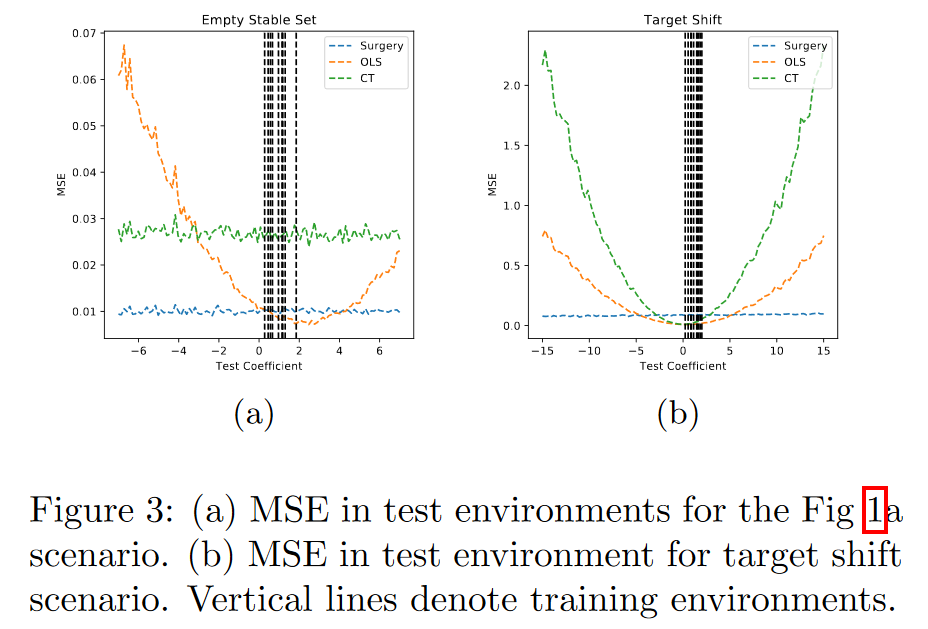
\includegraphics[scale=0.45]{figures/exp1.png}

\note[]{
CT is an alternative prior method for obtaining stable estimators.


}
\end{frame}

\begin{frame}
\frametitle{Bike Rentals}
We wish to predict hourly bike rentals ($R$), on the basis of temperature $T$, feeling temperature $F$, wind speed $W$, and humidity $H$.

\begin{center}
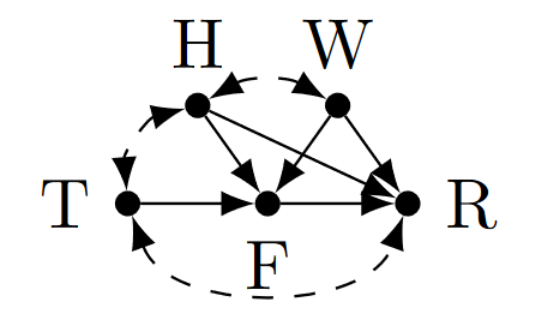
\includegraphics[scale=0.5]{figures/admg.png}
\end{center}

The data (over 2 years) is partitioned by season and year to create environments with different mechanisms. The mutable mechanisms are assumed to be $M = \{H, T, W\}$.
\end{frame}

\begin{frame}
\frametitle{Bike Rentals}
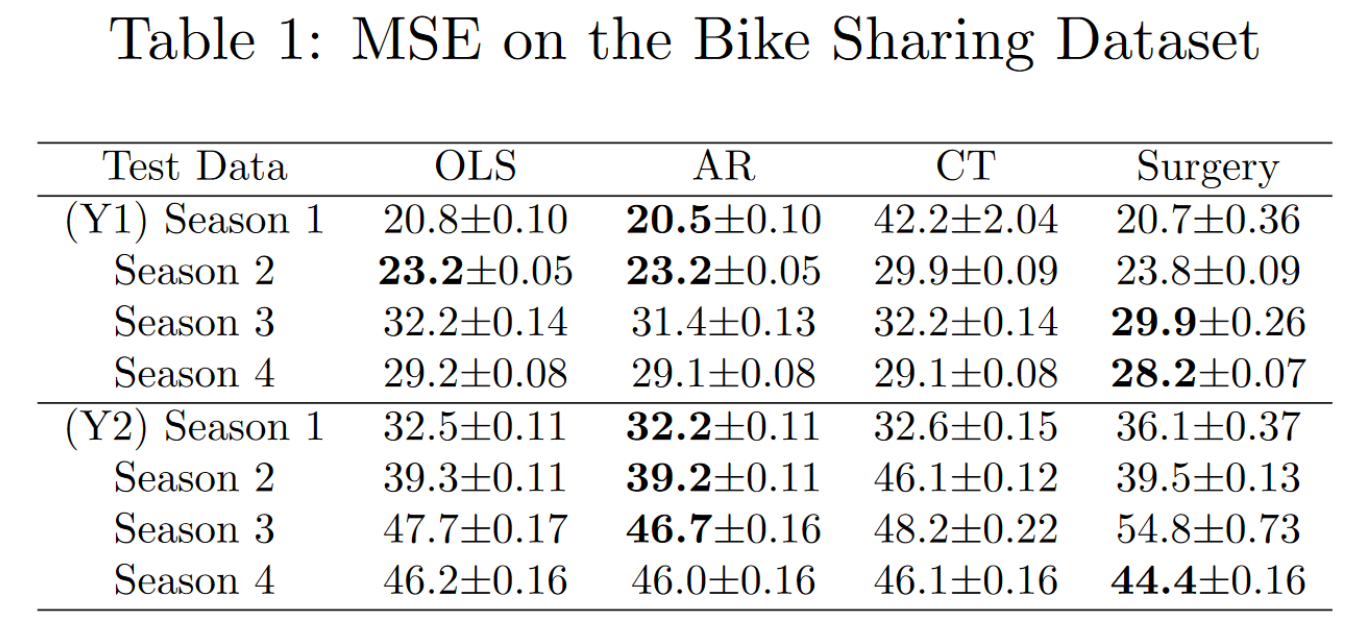
\includegraphics[scale=0.32]{figures/tab.png}

\note[]{

When  the  OLS  MSE  is  high  (sea-sons 3 and 4 in each year), Surgery tends to outper-form it which we attribute to Surgery’s stability.  Wealso see that CT tends to perform poorly which lendssome credibility to our hypothesized selection diagramwhich  dictates  that  no  stable  pruning  estimator  ex-ists.   AR’s  very  good  performance  is  expected,  sincethe shift-perturbation assumption seems reasonable inthis problem.  However,  AR requires tuning of a hy-perparameter for the maximum magnitude shift per-turbation  to  protect  against  which  is  less  preferablethan stable estimators such as surgery in safety criticalapplications when the target environment is unknownand could be very different from the source.
}
\end{frame}

\section{Concluding thoughts}

\begin{frame}
\frametitle{Proactive robustness, formalized}

Recall that we wish to predict $Y$ from $X$, in a way that achieves good performance over all environments. One possible way to formulate this is to be adversarial over environments:

$$\min_{f} \max_{e} \mathbb{E}_e \left[L(f(X), Y)\right]$$

In the context of causal diagrams, we can write this as a maximum over settings of the mutable variables $M$:

$$\min_{f} \max_{m} \mathbb{E}_{p(\cdot|do(M=m))} \left[L(f(X), Y)\right]$$

This means that the optimal predictor $f$ should achieve \textbf{uniform risk} over the possible settings.
\end{frame}

\begin{frame}
\frametitle{Proactive robustness, formalized}
\framesubtitle{Example}
\begin{center}
\tikz{ %
        \node[obs] (Z) {$Z$} ; %
        \node[obs, left=of Z, yshift=-2cm] (X) {$X$} ; %
		\node[obs, left=of X, yshift=2cm] (Y) {$Y$};
		\node[factor, yshift=1cm] (S) [label=$S$] {};  
        
        \edge {S} {Z} ; %
        \edge {Y} {Z} ;
        \edge {Y} {X} ;
        \edge {Z} {X} ;
      }
      \end{center}
      
$$\min_{f} \max_{z} \int \int L(f(X, Z), Y) p(Y) p(X|Y, Z) dx dy$$

Stable estimators are not necessarily optimal...
\end{frame}

\begin{frame}
\frametitle{Conclusion}

\begin{itemize}
	\item In many scenarios, it is desirable to obtain a classifier which is \textbf{proactively} robust against distribution shift;
	\item Causal approaches which take into can more accurately model unreliability in the DGP;
	\item There are still interesting questions regarding the tradeoff between performance/stability, and whether there might be other causal methods which can improve upon graph surgery
\end{itemize}
\end{frame}




\bibliographystyle{apalike}
\bibliography{L3citations}
\end{document}

